\documentclass[11pt]{article}
\usepackage{fullpage}
\usepackage{graphicx}
\usepackage{hyperref}
\begin{document}

\title{Homework 1 -- Mesh Simplification and Progressive Meshes}
\author{Gabe Fierro and Graham Tremper}
\date{\today}
\maketitle

\section{Introduction}

A video demonstration of our solution can be found here:
\begin{center}
\href{http://www.youtube.com/watch?v=DfLkut3YniE}{http://www.youtube.com/watch?v=DfLkut3YniE}.
\end{center}
The code for our solution is publicly available on Github:
\begin{center}
\href{https://github.com/gtremper/MeshSimplification}{https://github.com/gtremper/MeshSimplification}.
\end{center}
The code was compiled using Boost 1.53.0 and GLM 0.9.4.1 on Mac OS X 10.7.4 and
10.8.2. To compile, run \verb`make` from the \verb`MeshSimplification` directory. The OFF models
are included in the \verb`Models` directory. The compiled binary, \verb`viewer`,
accepts the path to a model as the only argument, and can be run as follows:

\begin{center}
  \verb`prompt> ./viewer Models/teapot.off`
\end{center}

The up and down arrow keys will increase and decrease the number of edges in
the displayed mesh. Initially, the viewer will change the mesh at the rate of 1
edge collapse each time the up or down arrows are pressed. This rate can be
increased or decreased by an order of magnitude by using the right and left
arrows respectively. For example, to simplify a model by 1000 edges at a time,
press the right arrow 3 times to increase from 1 to 10 to 100 to 1000 edges,
then press the down arrow to start collapsing edges.

To toggle displaying the wireframe of the model, press \verb`f`. Press \verb`p`
to toggle between flat and smooth shading. Clicking and dragging the mouse will
move the model, and pressing \verb`m` will slowly rotate the model.

\section{Half Edges}

We chose the half edge data structure to consist our meshes over the obvious
alternatives of winged edge and adjacency lists due to its advantages in
simplicity, size and speed. We consider an edge to be sourced at a given
vertex, and directed in an anti-clockwise manner corresponding to the canonical
ordering for the representation of a triangle. Given this assumption, a half
edge, at minimum, keeps track of the source vertex of the edge, the next
(following) edge in anti-clockwise order, and the symmetric edge. The symmetric
edge is defined to be the edge sourced at the destination vertex for a given
edge, pointing towards the source vertex of the initial edge. Many
implementations of half edges also store which face contains that edge, but for
our purposes, this additional pointer is unnecessary, and the space can be
better utilized to store the previous edge.

\begin{figure}[htb]
\begin{center}
  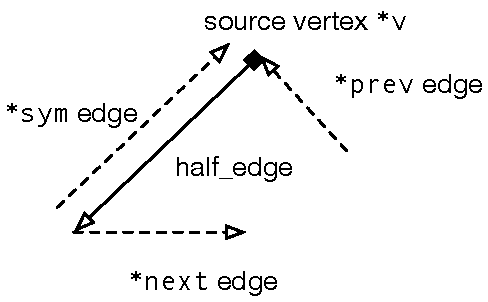
\includegraphics{figs/half_edge-data-structure}
\end{center}
\caption{Half Edge Data Structure}
\end{figure}


Our version of the half edge data structure is as follows:

\begin{verbatim}
    struct half_edge {
        int v; // index into the list of all vertices
        half_edge *prev, *next, *sym; // pointers to related edges
        edge_data* data; // bookkeeping for edge collapse
        int index; // bookkeeping for vertex splits
    };
\end{verbatim}

The half edge data structure allows for efficient and localized methods of
obtaining the relations between vertices and edges. Obtaining the two endpoints
for a collapsing edge is a constant time operation.  Obtaining the neighbors
for a vertex is linear in the number of edges that touch the vertex, meaning
that an edge collapse is almost entirely localized so that the entire mesh does
not need to be updated after each operation. Most of this is made possible by
the use of the \verb`*prev`, \verb`*next` and \verb`*sym` pointers; by chaining
together half edges, we can access arbitrary information without the need to
traverse a vector or other slow data structure.

The vertices themselves are allocated during the construction of the mesh and
are stored in a vector, allowing for amortized constant time append operations
for the vertices generated during edge collapses. Each half edge keeps track of
its source vertex by means of an integer index into this vector, eliminating
any pointer work that must be done to update each edge's new vertex after an
edge collapse. Each of the neighboring edges simply has its vertex index set to
the last item in the vector -- the edge collapse vertex.


\section{Edge Collapses}

The task of collapsing an edge can be separated into several discrete sub-tasks. After finding the 
least-cost edge (see the section on Quadric Simplification, below, for details), we find the neighboring
edges that share a vertex with either end of the edge to be collapsed. We compute the new vertex for
the two ends of the collapsed edge, then update the \verb`half_edge`s surrounding the new vertex
to ensure the consistency of mesh.

\begin{figure}[htb]
  \begin{center}
    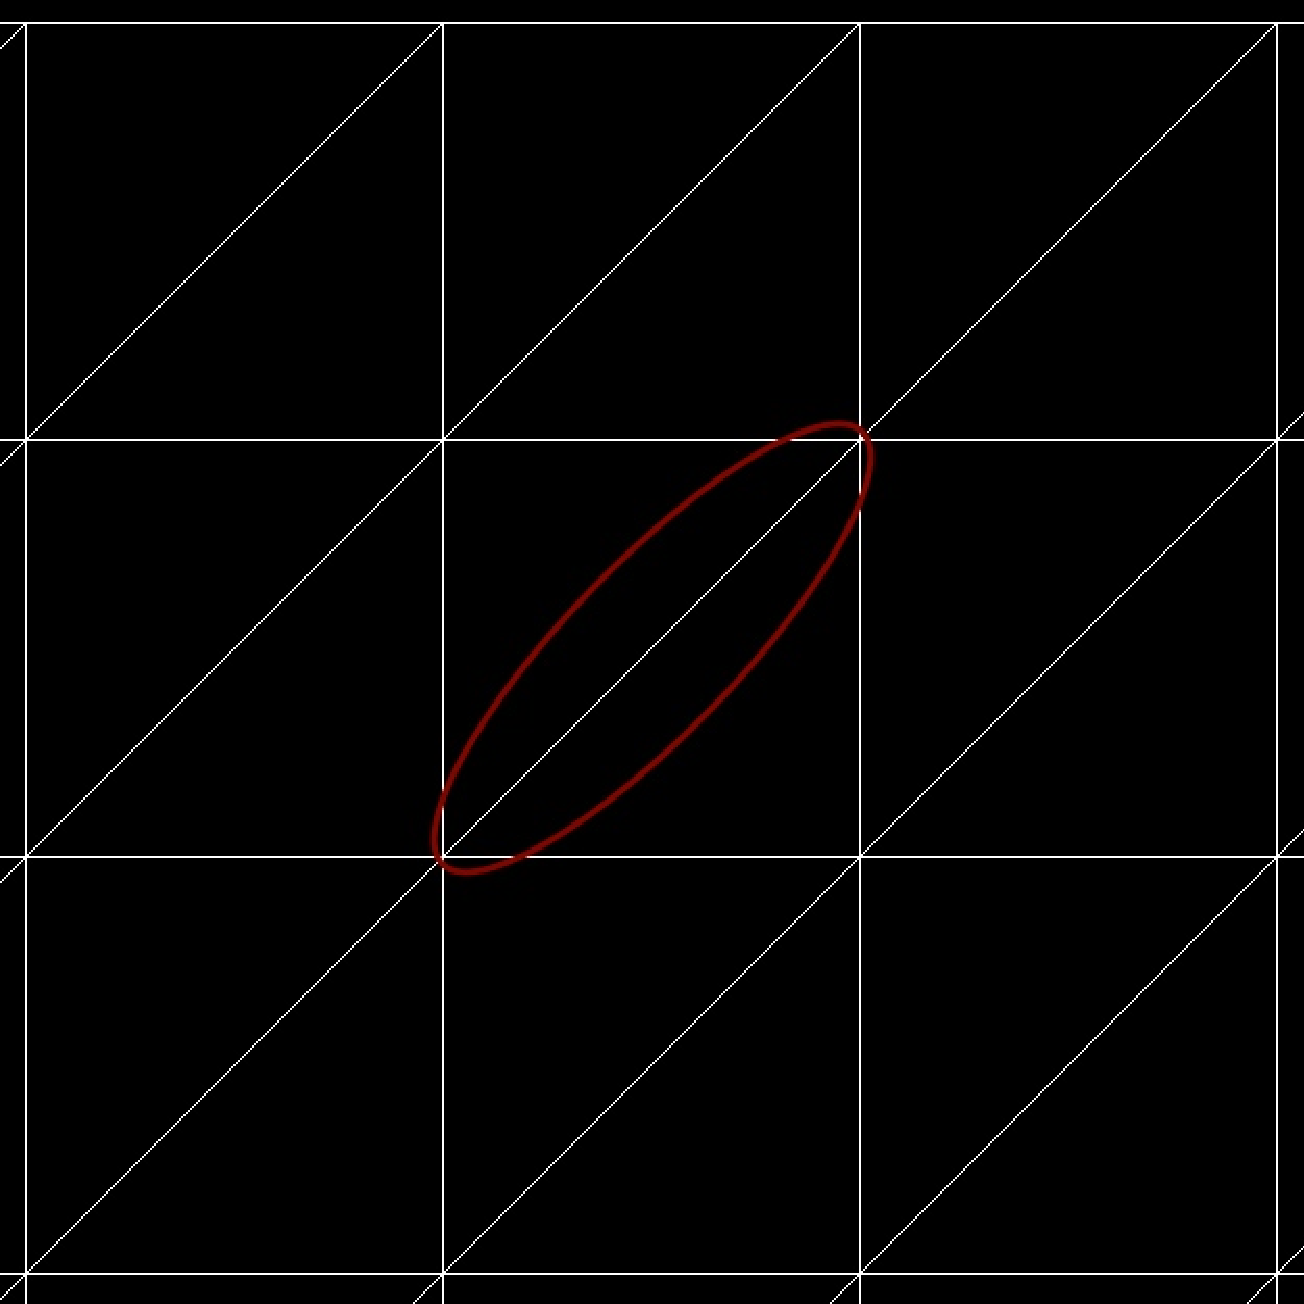
\includegraphics[width=.32\linewidth]{figs/ec1.pdf}
    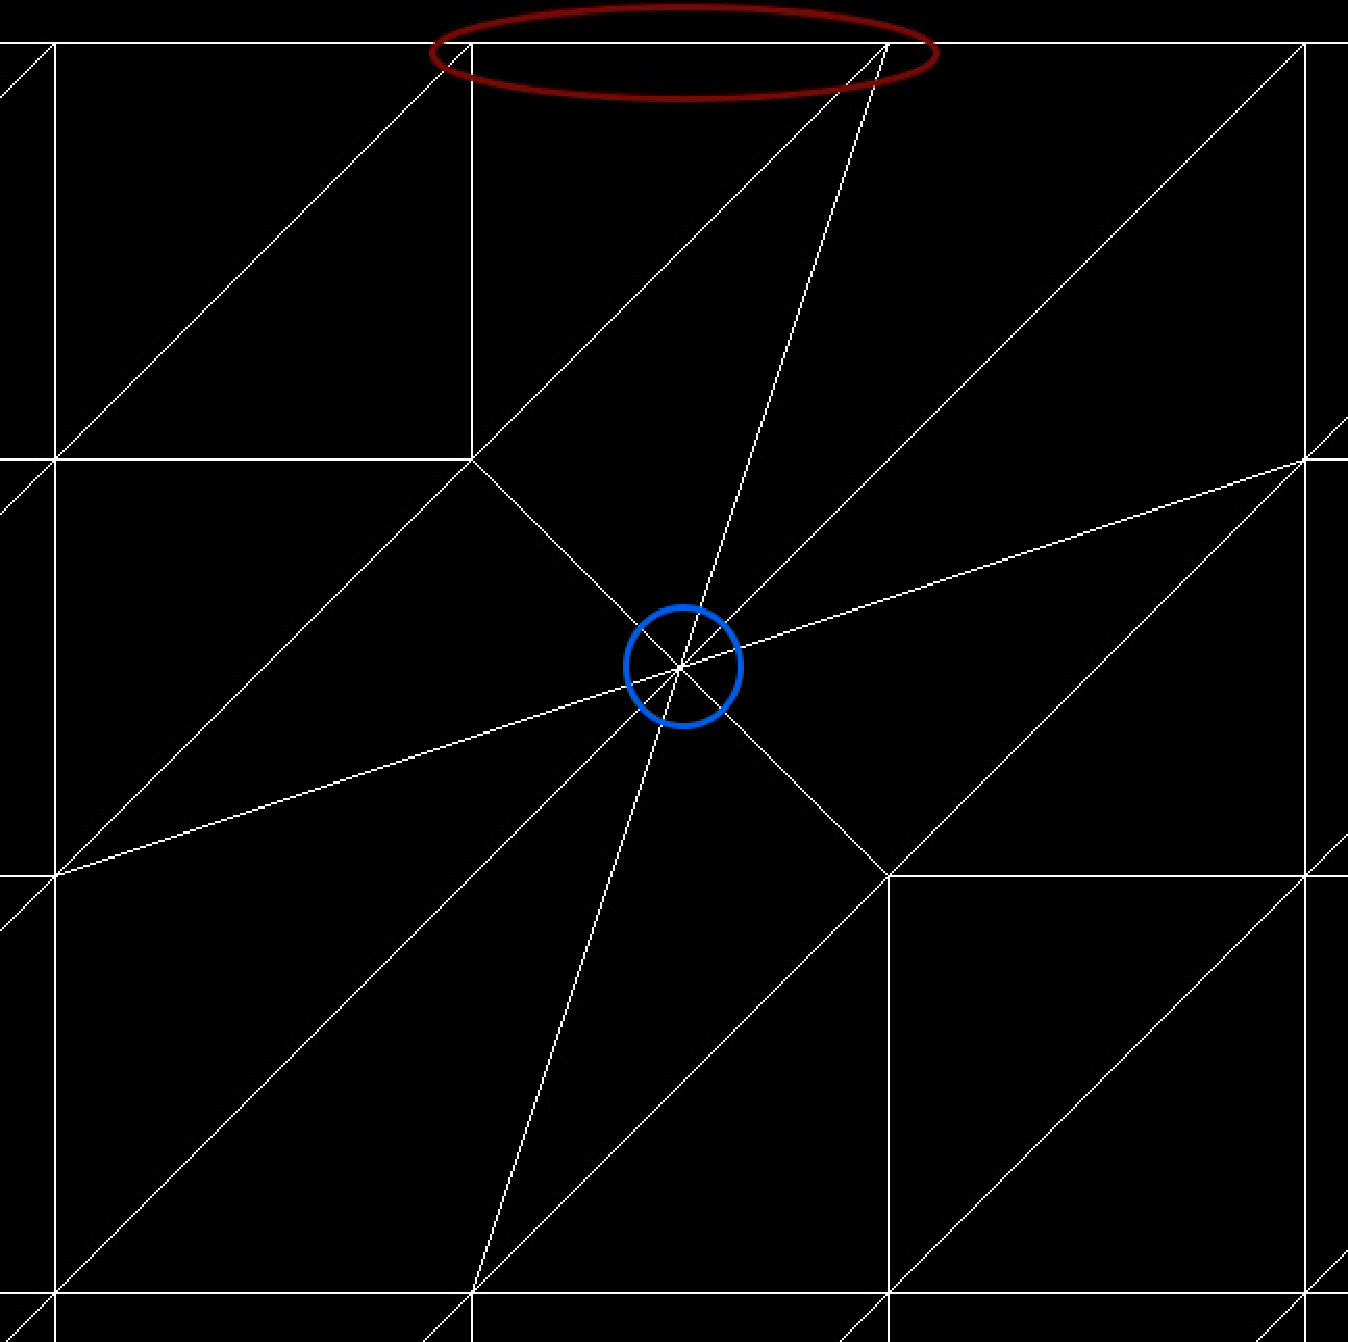
\includegraphics[width=.32\linewidth]{figs/ec2.pdf}
    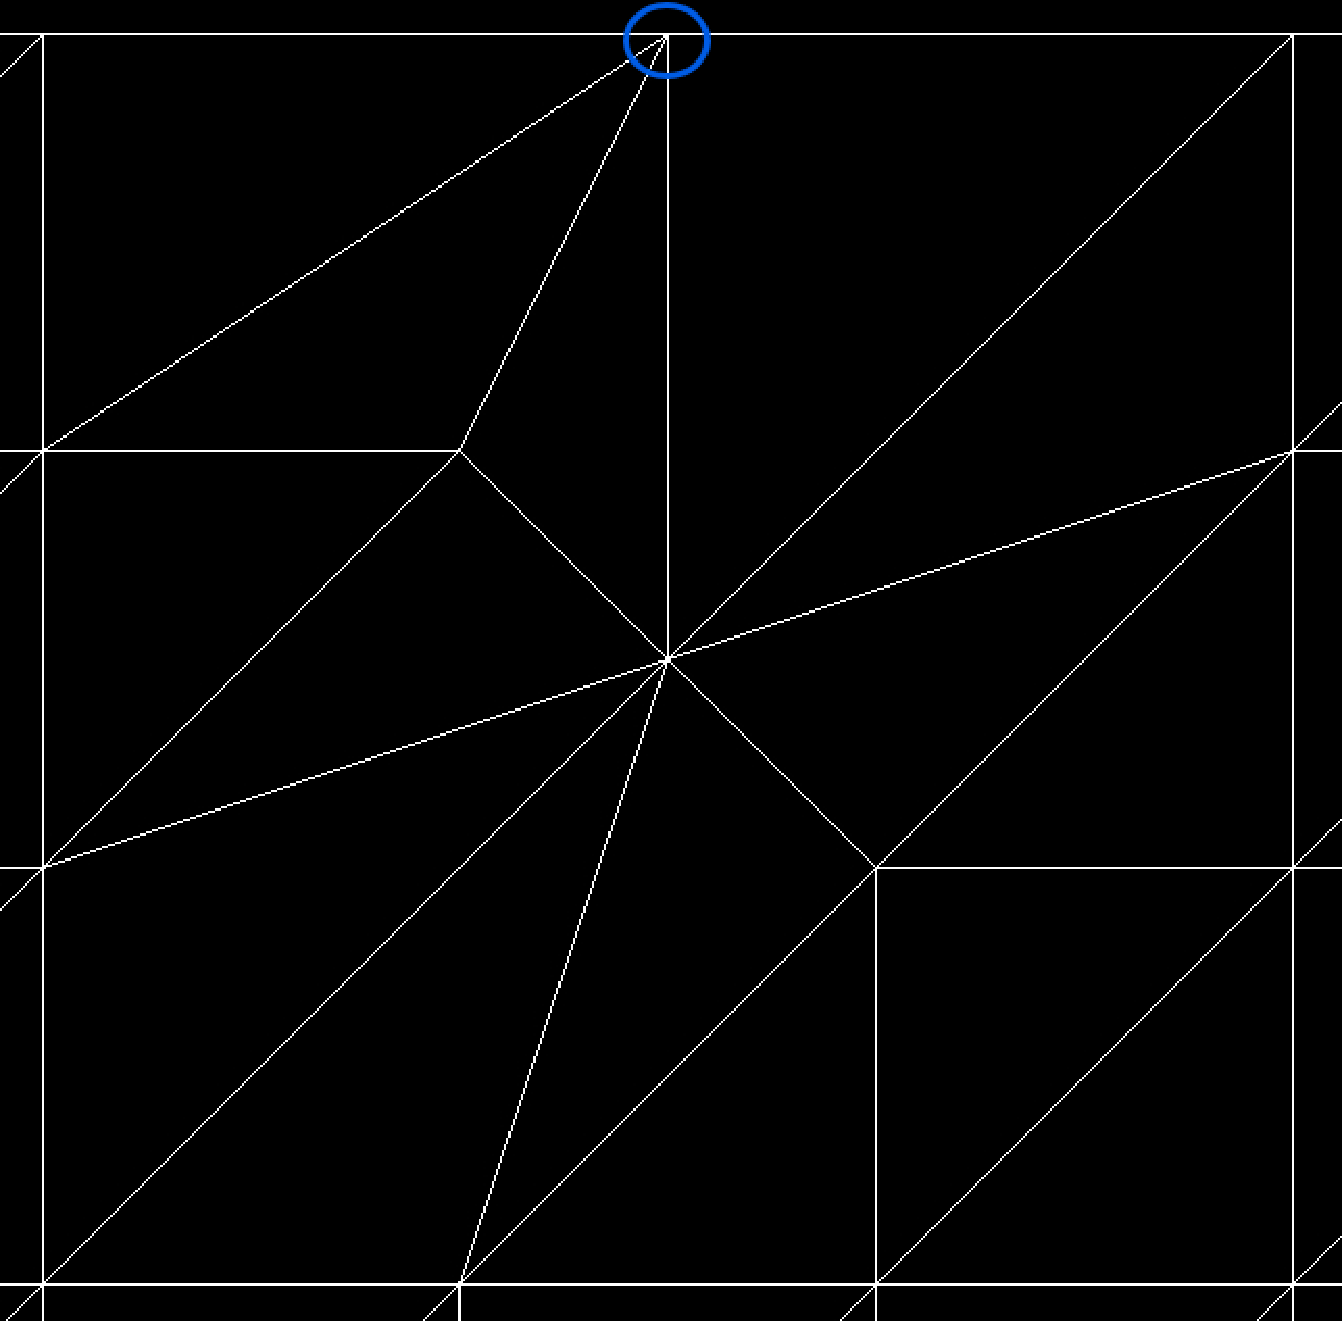
\includegraphics[width=.32\linewidth]{figs/ec3.pdf}
  \end{center}
\caption{Two successive edge collapses. The edge collapse is circled in red, and the resulting vertex
is circuled in blue. Here, we can see an example of collapsing a fully surrounded edge followed by
an example of collapsing a bordering edge. Edges highlighted in green must be traversed and have their
source vertex updated.}
\end{figure}

\subsection{Finding Neighboring Edges}

The basic paradigm for obtaining the neighboring edges for each of the two
vertices consisting an edge begins with finding an edge that contains one of
the indicated vertices as its source vertex, and then following a chain of
pointers to loop around the vertex. This is appropriate for manifold surfaces,
in which every single edge has a corresponding symmetric edge, but fails for
more complex surfaces, in which edges may not have a symmetric edge and in
which neighbors may not be traversed contiguously.

The base method for obtaining the edges that share a source vertex is:

\begin{verbatim}
    /* start with half_edge* he */
    half_edge* loop = he->prev->sym;
    while (loop != he) {
        neighbors.push_back(loop);
        loop = loop->prev->sym;
    }
\end{verbatim}

Obviously, this will break in cases where an edge has a NULL \verb`sym`,
indicating that it is on the edge of a non-manifold mesh. To account for these
problems, we implement different traversal functions for each of the cases where a
relevant symmetric edge might be null:

\begin{itemize}
    \item \verb`he->sym == NULL`
    \item \verb`he->prev->sym == NULL`
    \item \verb`he->next->sym == NULL`
\end{itemize}

\subsection{Updating Edge Pointers}

One of the trickier parts of using the half edge data structure is updating the
\verb`half_edge` pointers during an edge collapse. Basically, the
\verb`half_edges` corresponding to the degenerate faces are removed, and the
``sym'' pointers of neighboring edges are updated. In addition to the two
implicit degenerate faces from an edge collapse, we also remove ``fins'' which
can become problematic later on. Unfortunately, there is at least one ``edge''
case that we have not been able to detect and correct for. This causes the mesh
data structure to rarely become corrupted on some of the larger models. For
example, the ``brain'' model will crash if collapsed more than half way. This
is a rare occurrence, though, and most of the models are unaffected.

\begin{figure}
  \begin{center}
    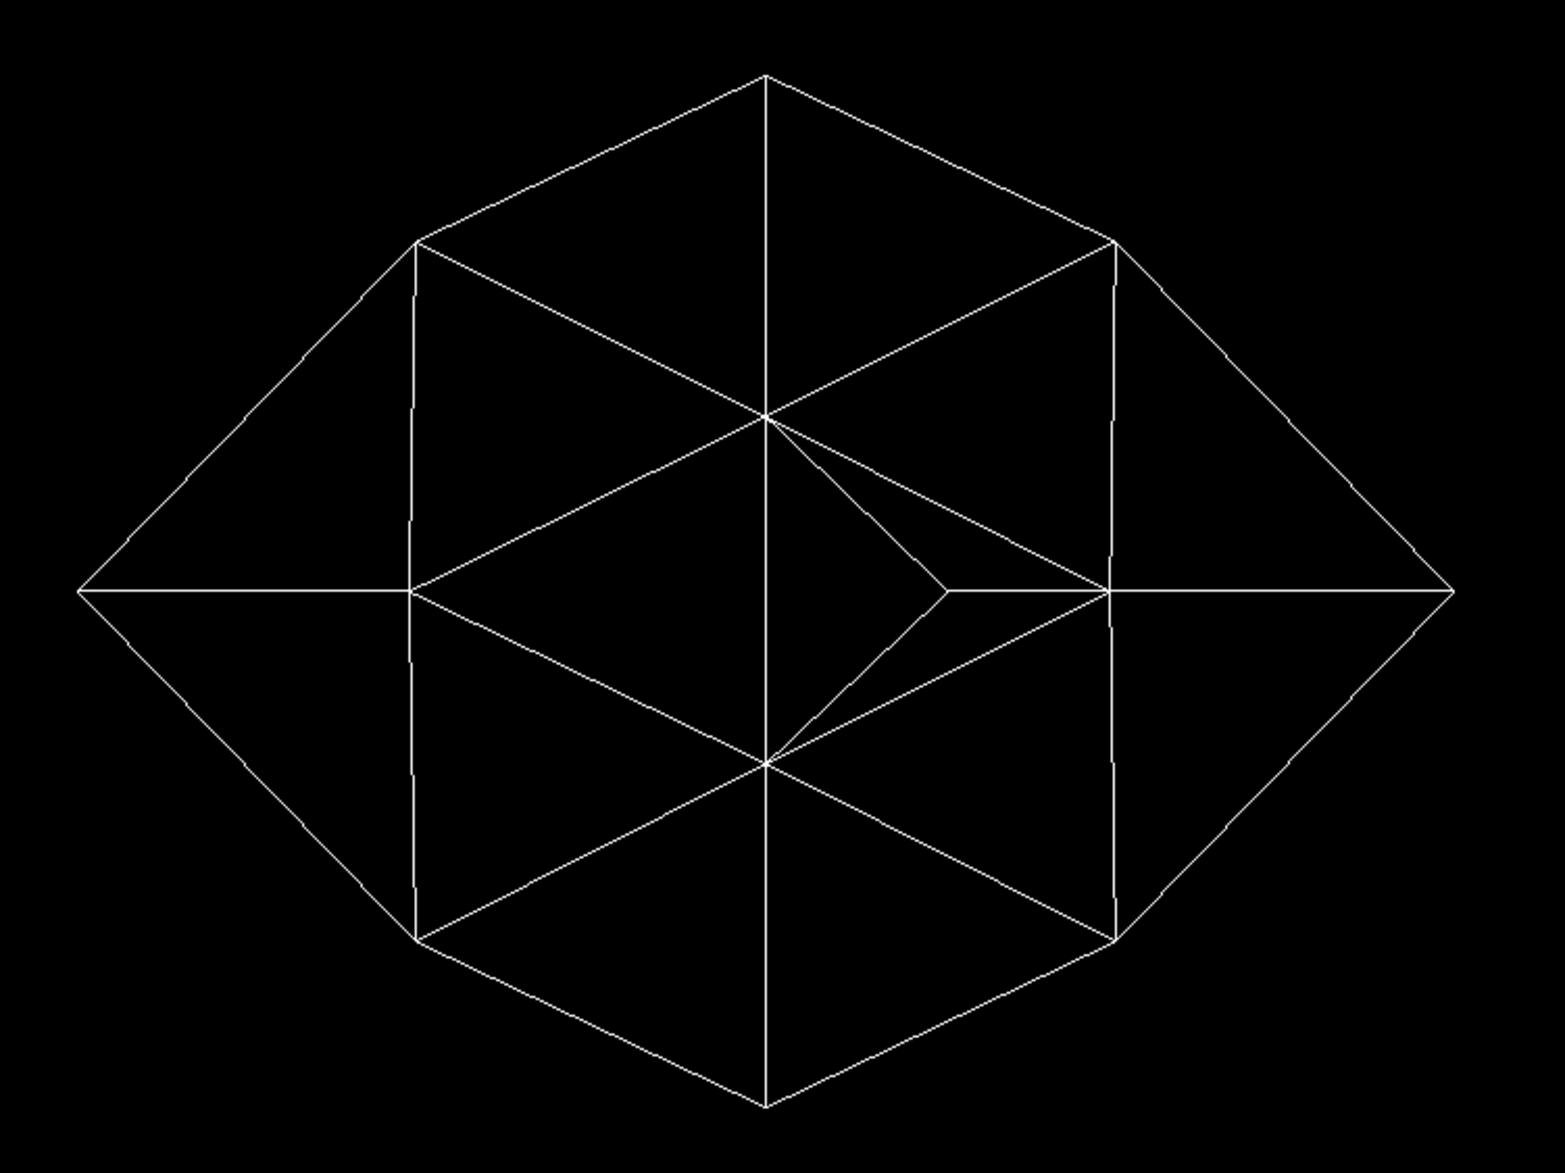
\includegraphics[width=.30\linewidth]{figs/fin1}
    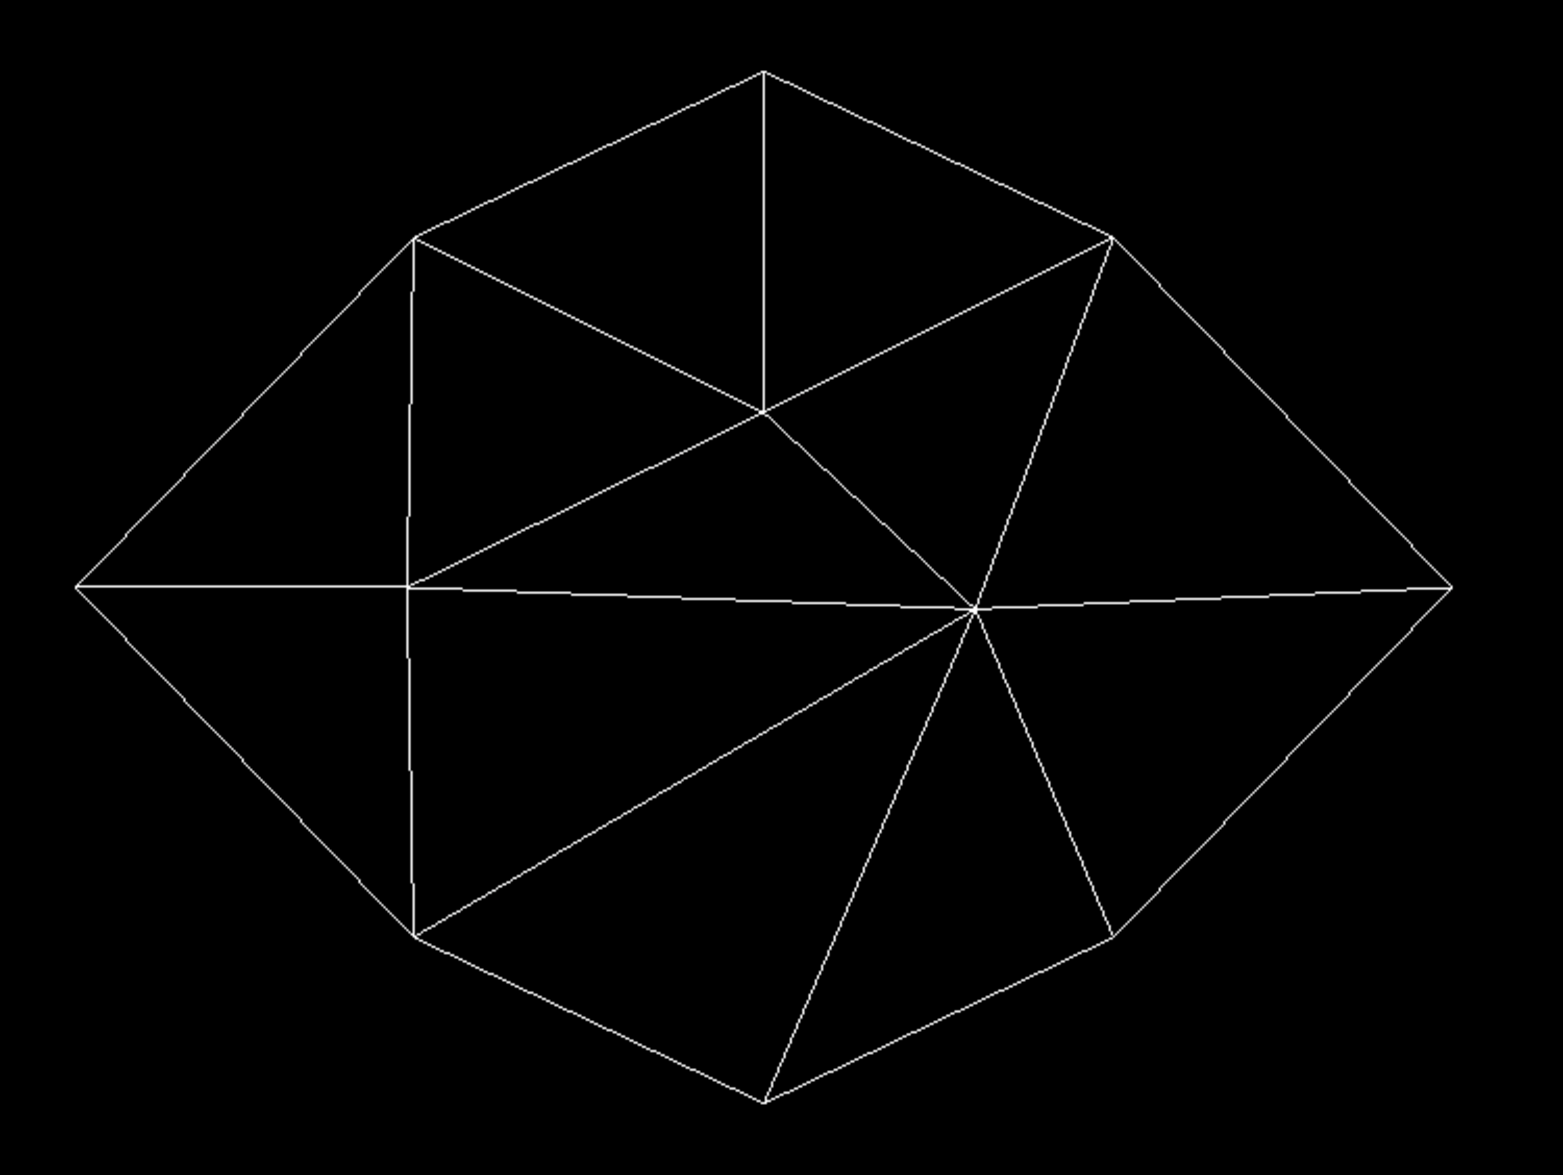
\includegraphics[width=.30\linewidth]{figs/fin2}
  \end{center}

  \caption{The left figure shows a triangle with two ``fins''. When the edge is collapsed, the two extra ``fins'' are collapsed, removing a total of four triangles.}

\end{figure}

\section{Quadric Simplification}

Every vertex has 10 floats that represent the quadric Q matrix. For every edge in the mesh, an \verb`edge_data` object is created (one for every pair of symmetric edges) which stores the optimum merge point for the two vertices and the associated quadric error. We also decided to add a small random $\epsilon$ to each quadric error. This ``jitter'' helps evenly distribute the edge collapses when model is very dense. This prevents all of the zero error collapses from clustering in an undesirable pattern. As the quadric error for a collapse increases, this term becomes irrelevant. The \verb`edge_data` objects are then stored in a priority queue sorted by their quadric error. A handle to each of the objects in the in the priority queue is stored with the associated edge, so that modified edges can update their \verb`edge_data` object when the error is changed. To go down a level of detail, the edge at the top of the priority queue is collapsed, and and degenerate edges are removed from the queue. The Boost library implementation of a binomial heap was chosen for its constant time access of the next edge to be collapsed, and amortized logarithmic time for updating edges.

\section{Progressive Meshes}

\begin{figure}[ht]
  \begin{center}
    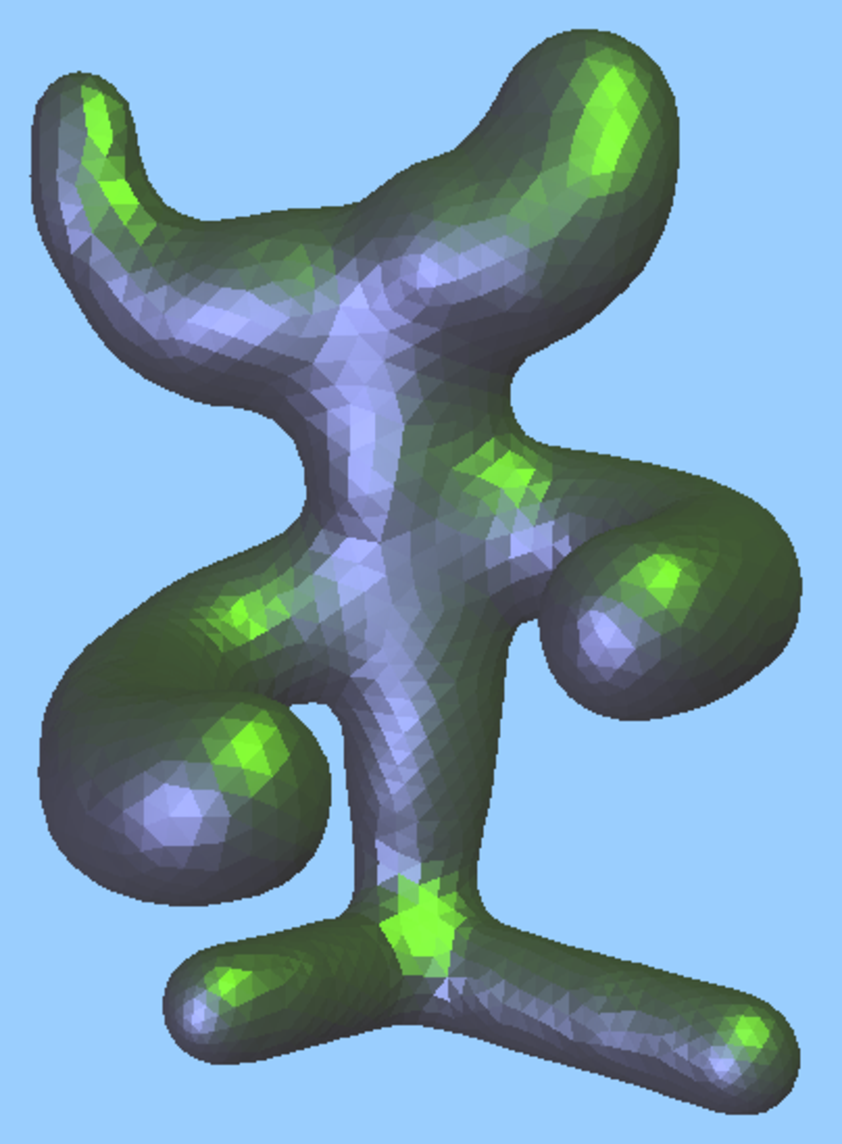
\includegraphics[width=.24\linewidth]{figs/moomoo7776}
    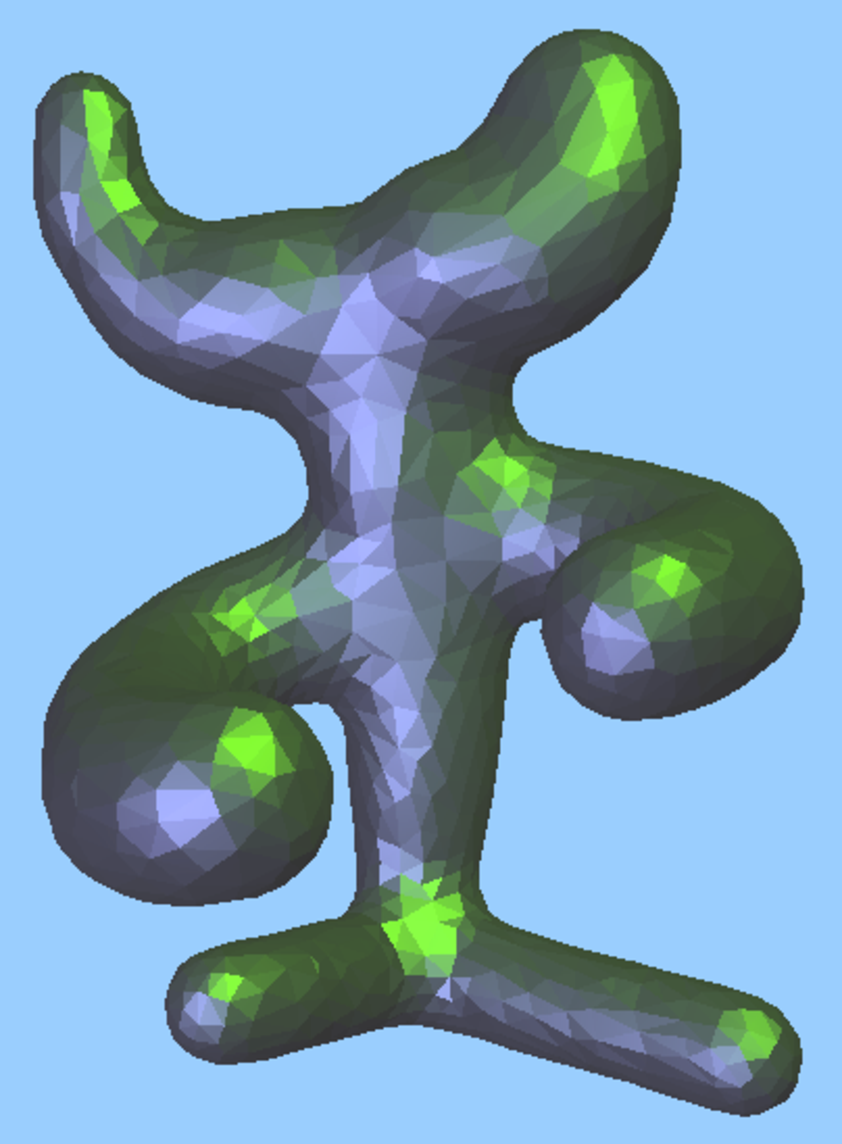
\includegraphics[width=.24\linewidth]{figs/moomoo3776}
    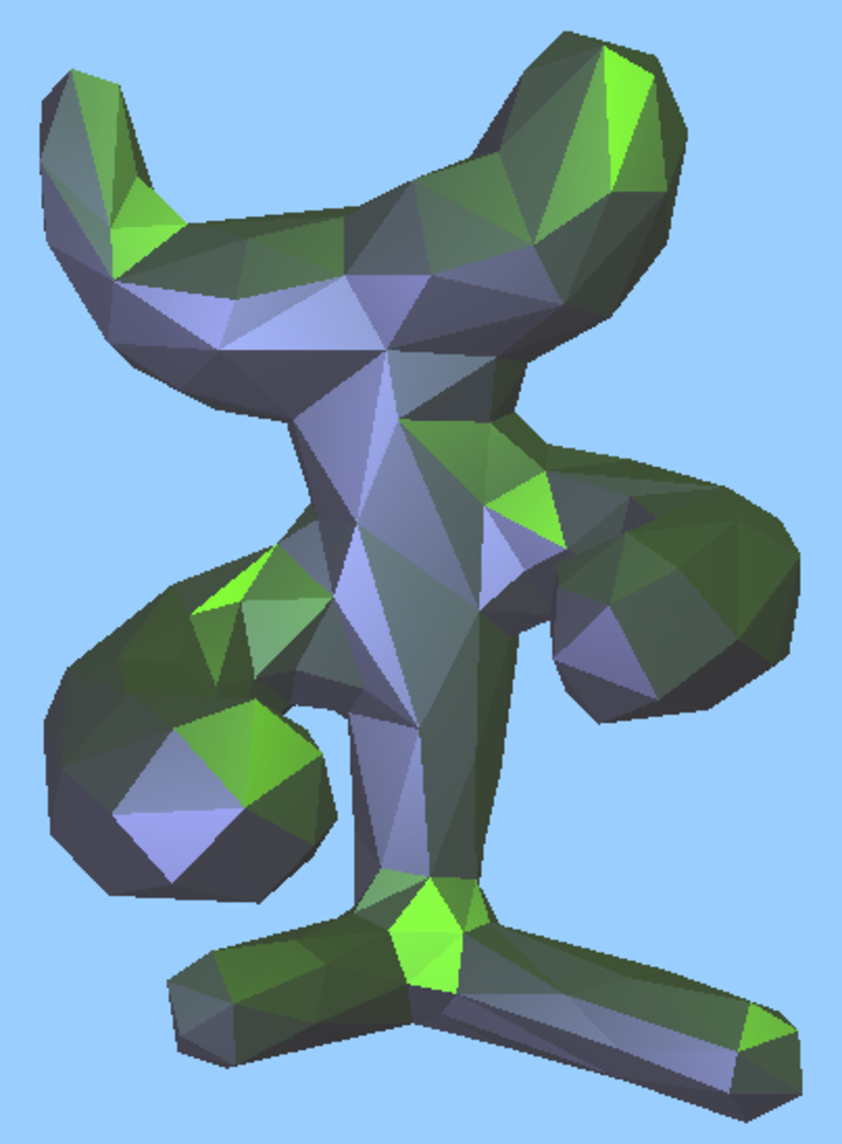
\includegraphics[width=.24\linewidth]{figs/moomoo460}
    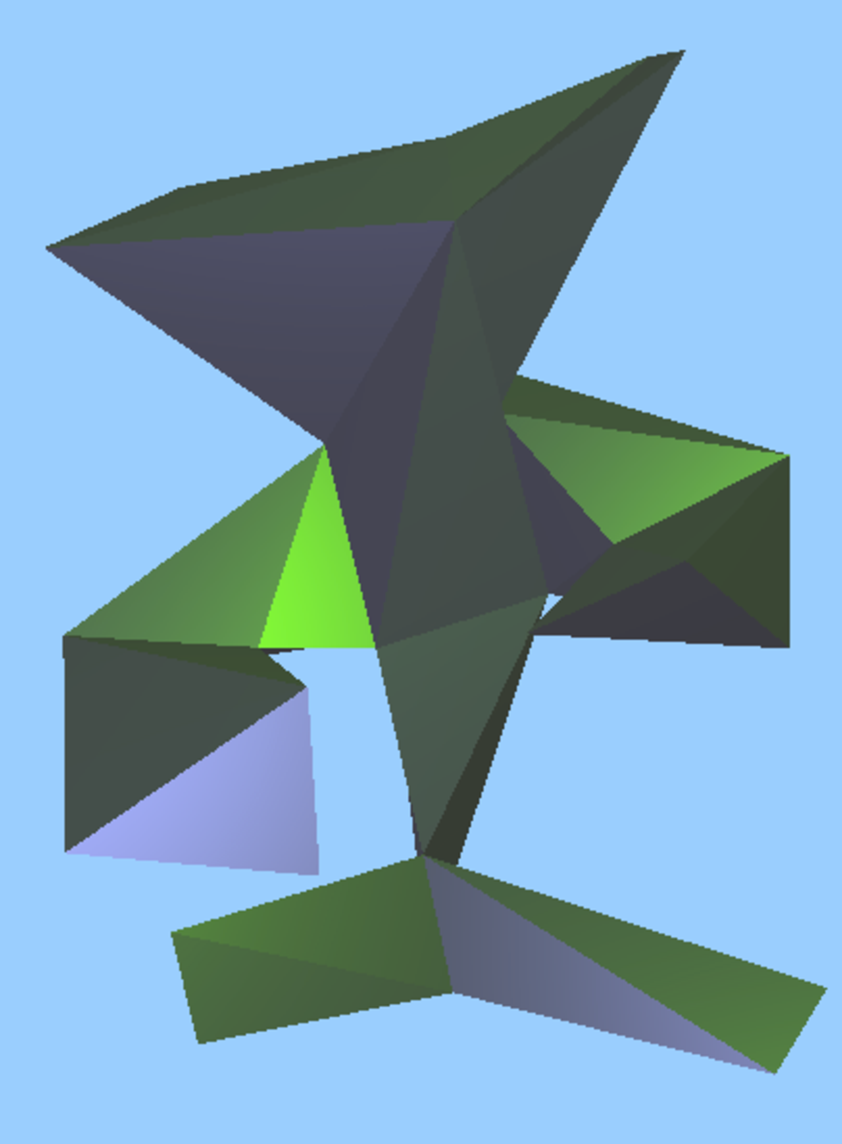
\includegraphics[width=.24\linewidth]{figs/moomoo58}
  \end{center}

  \caption{Here we can see several stages of progressive mesh simplification on
  the moomoo model. From left to right, 7776 faces (full model), 3776 faces, 460
  faces, 58 faces.}

\end{figure}

Objects are drawn using Vertex Buffer Objects (VBOs). After parsing all of the
vertices from the OFF file, new vertices are appended to the end of the vertex
when created during an edge collapse. This way, once all of the edges are
collapsed, we have calculated and stored all of vertices that are possible at
any level of detail. This makes switching between levels of detail very easy by
simply changing the indices in the element array buffer. This allows us to
simply store the changes in the indices for each level of detail. This is
implemented using a vector of \verb`collapse_data` objects which store the changes
need to move both up and down a level of detail.

\section{Armadillo Simplification}

Here, we present the simplification from the full armadillo model of over
345000 faces to 376.

\begin{figure}[ht]
  \begin{center}
    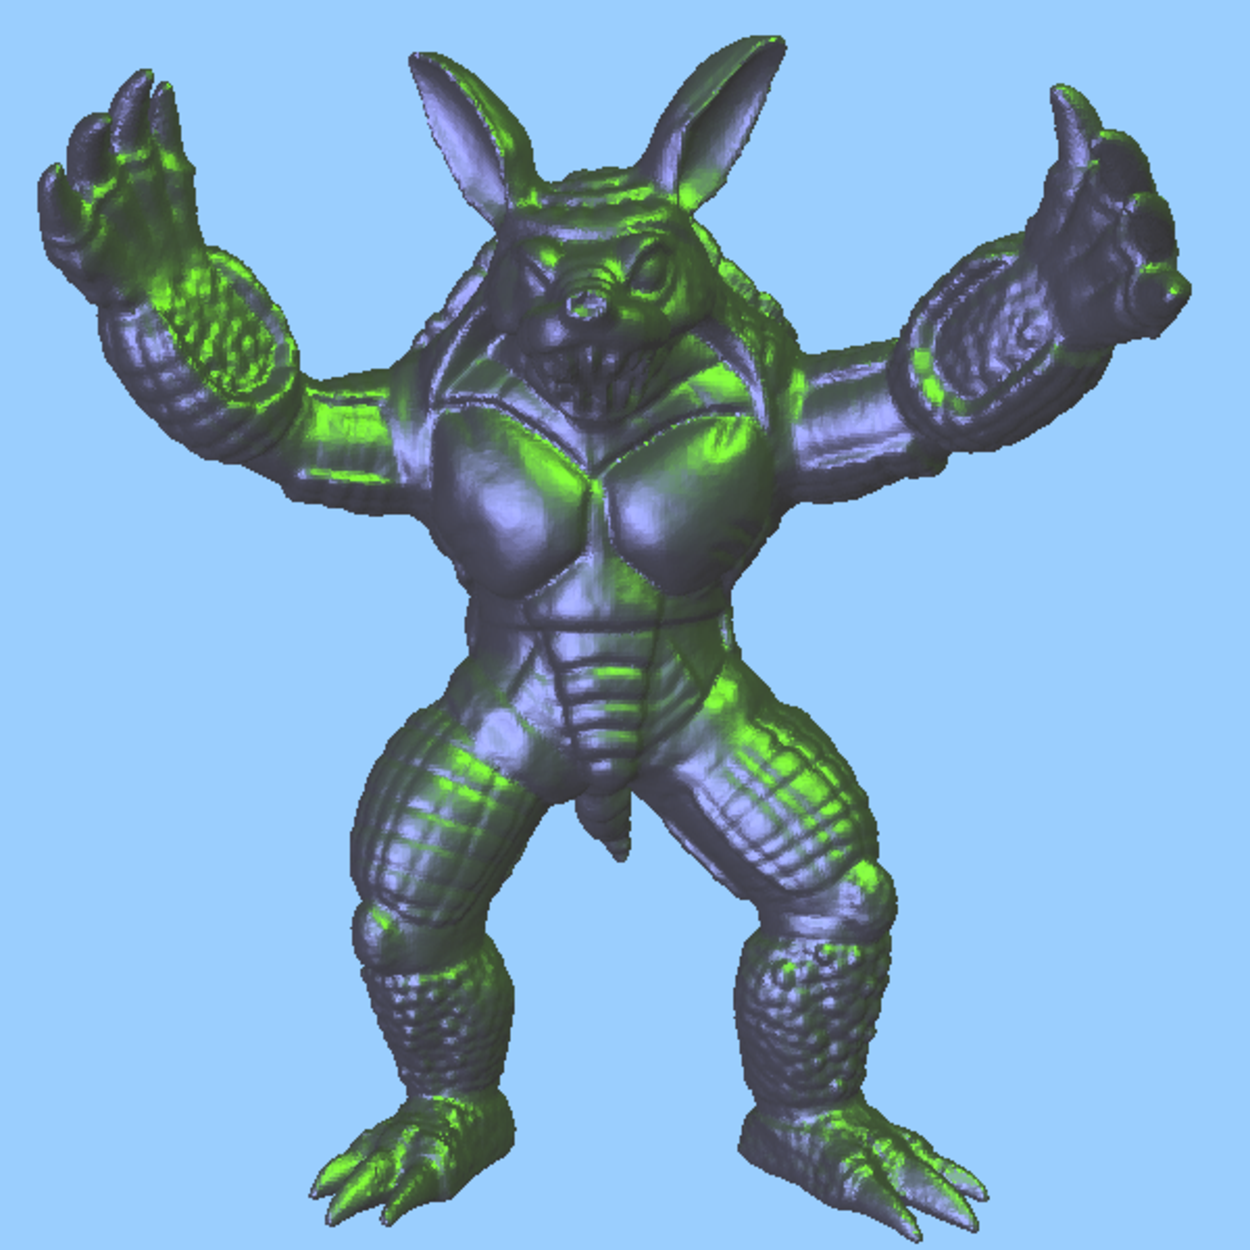
\includegraphics[width=.25\linewidth]{figs/armadillo345944}
    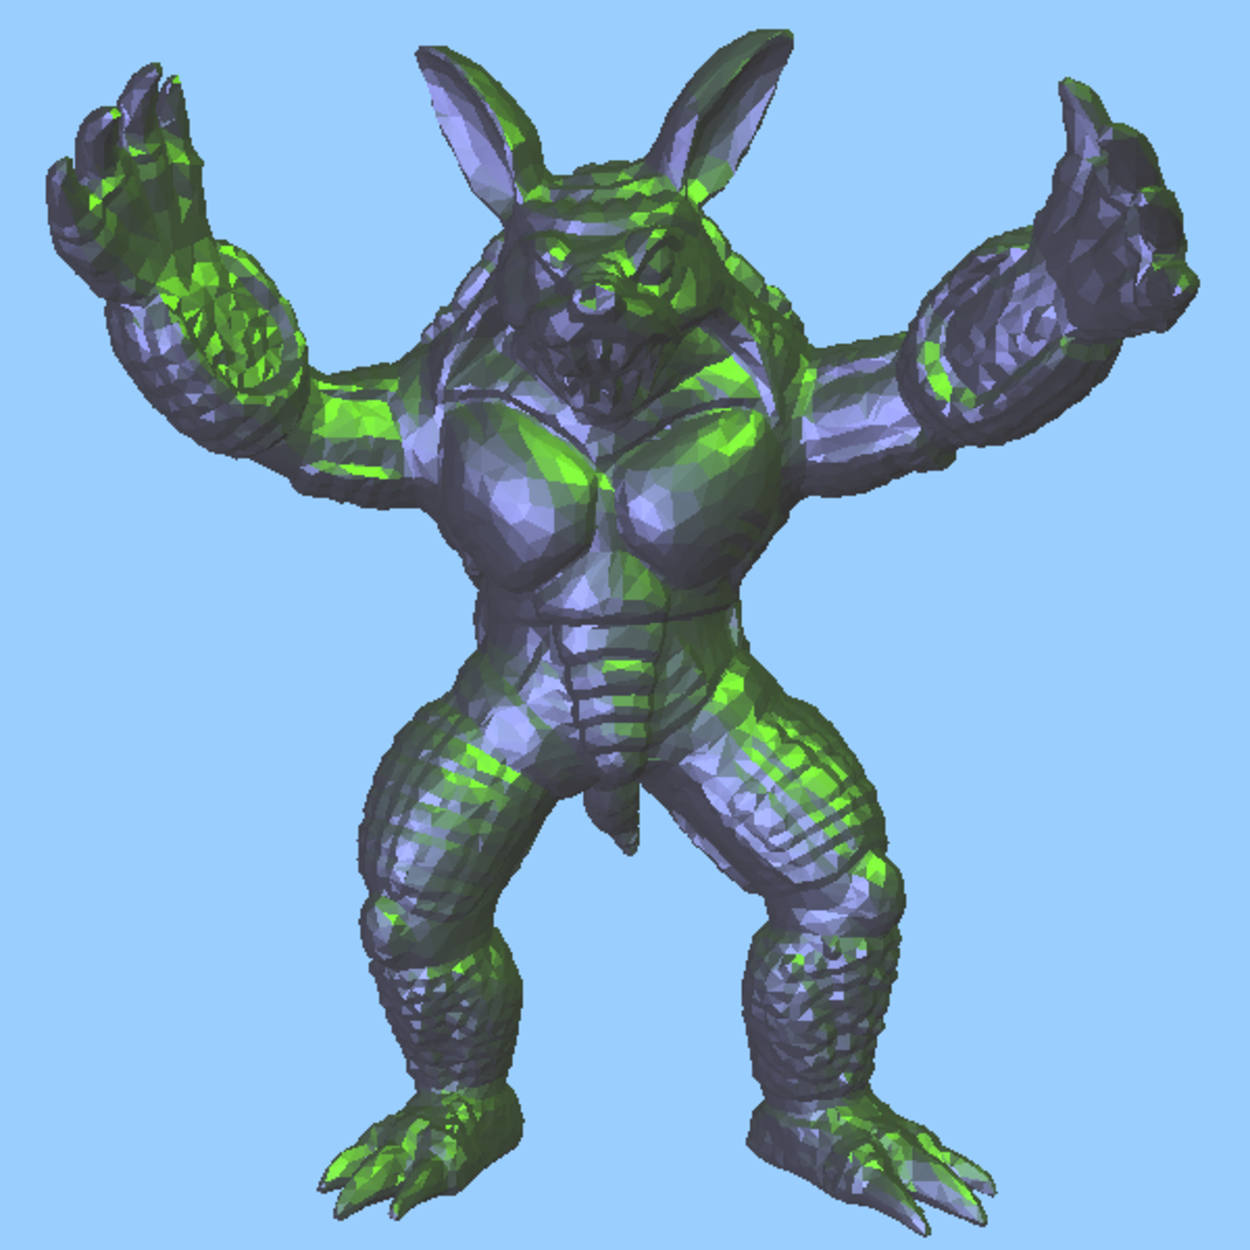
\includegraphics[width=.25\linewidth]{figs/armadillo23410}
    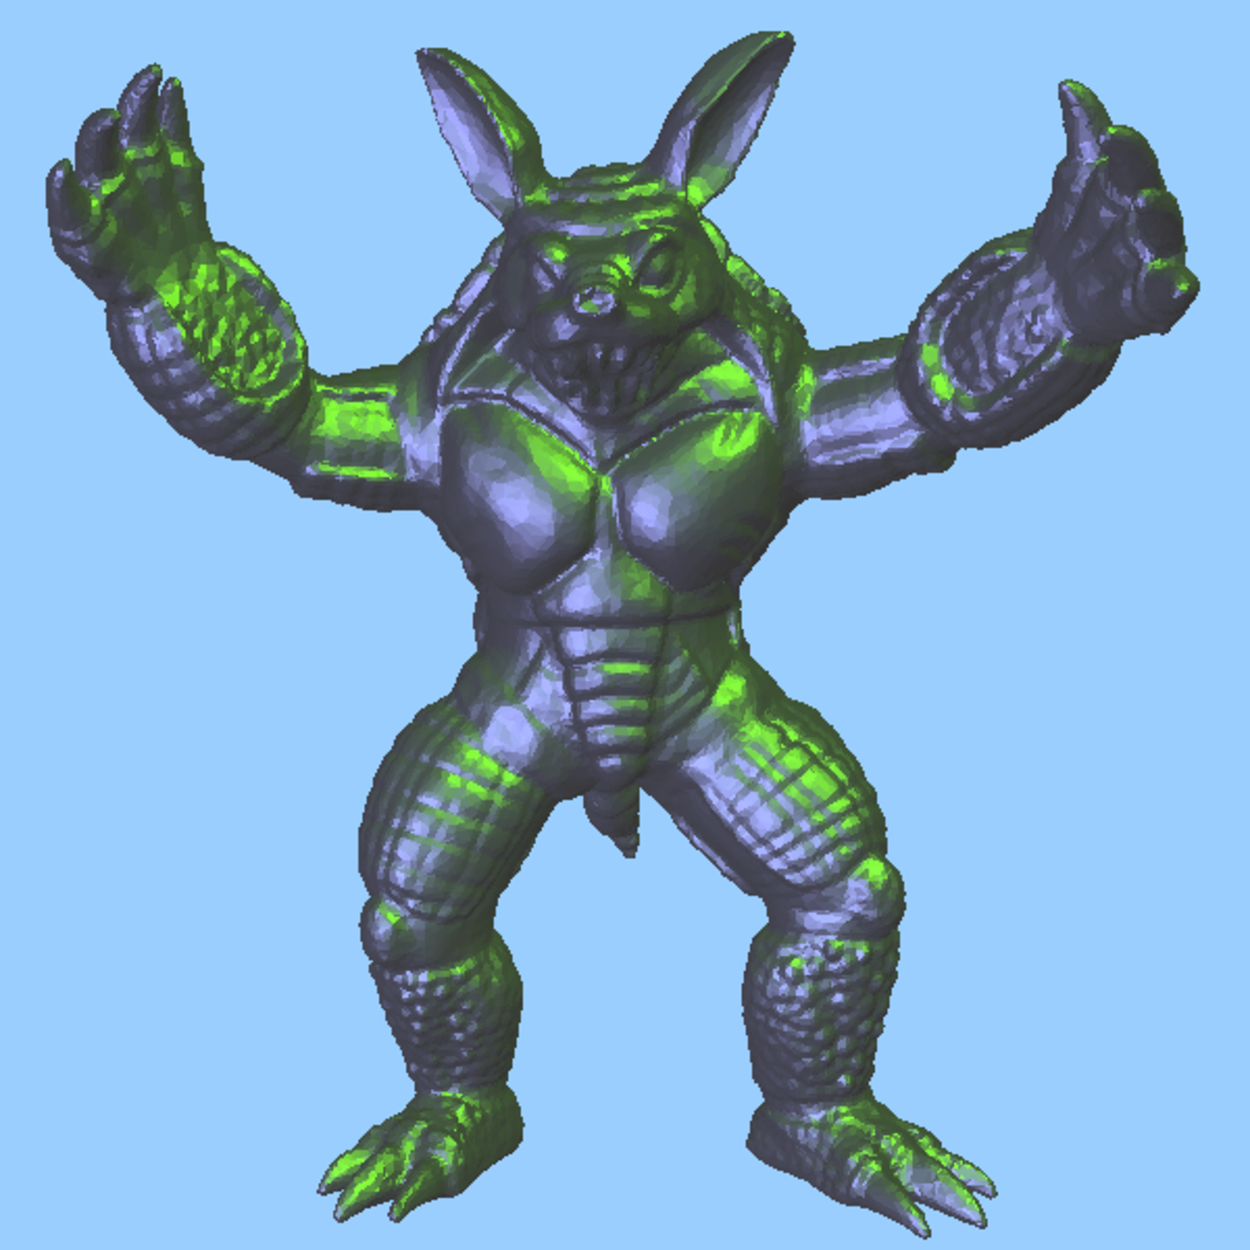
\includegraphics[width=.25\linewidth]{figs/armadillo83426}
    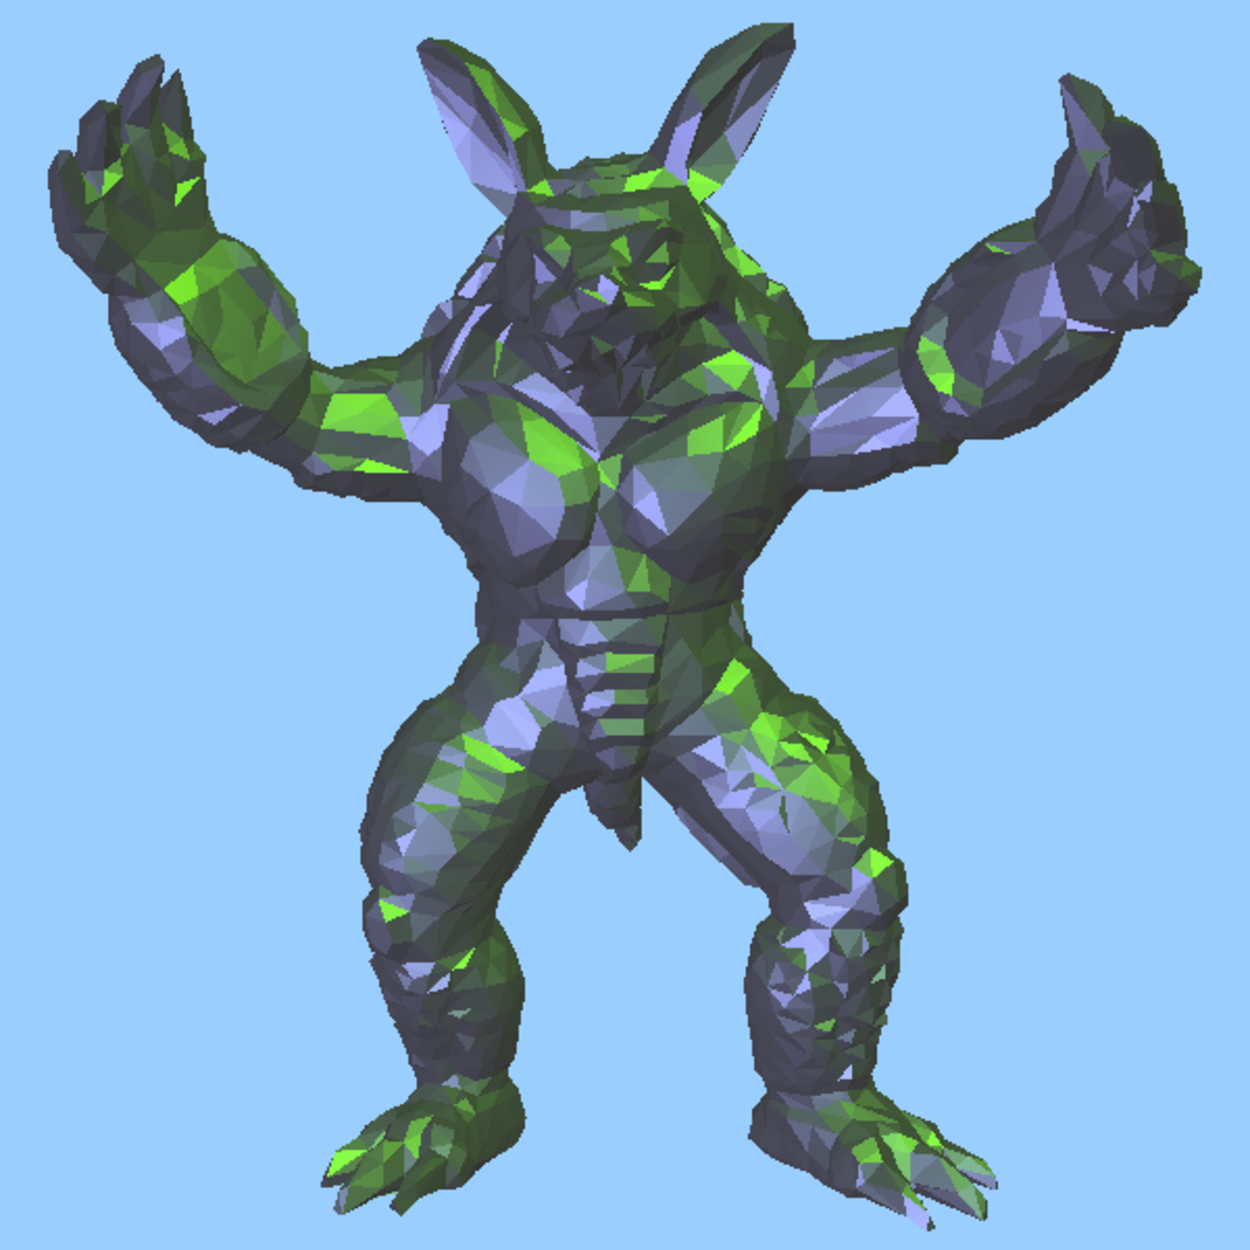
\includegraphics[width=.25\linewidth]{figs/armadillo6380}
    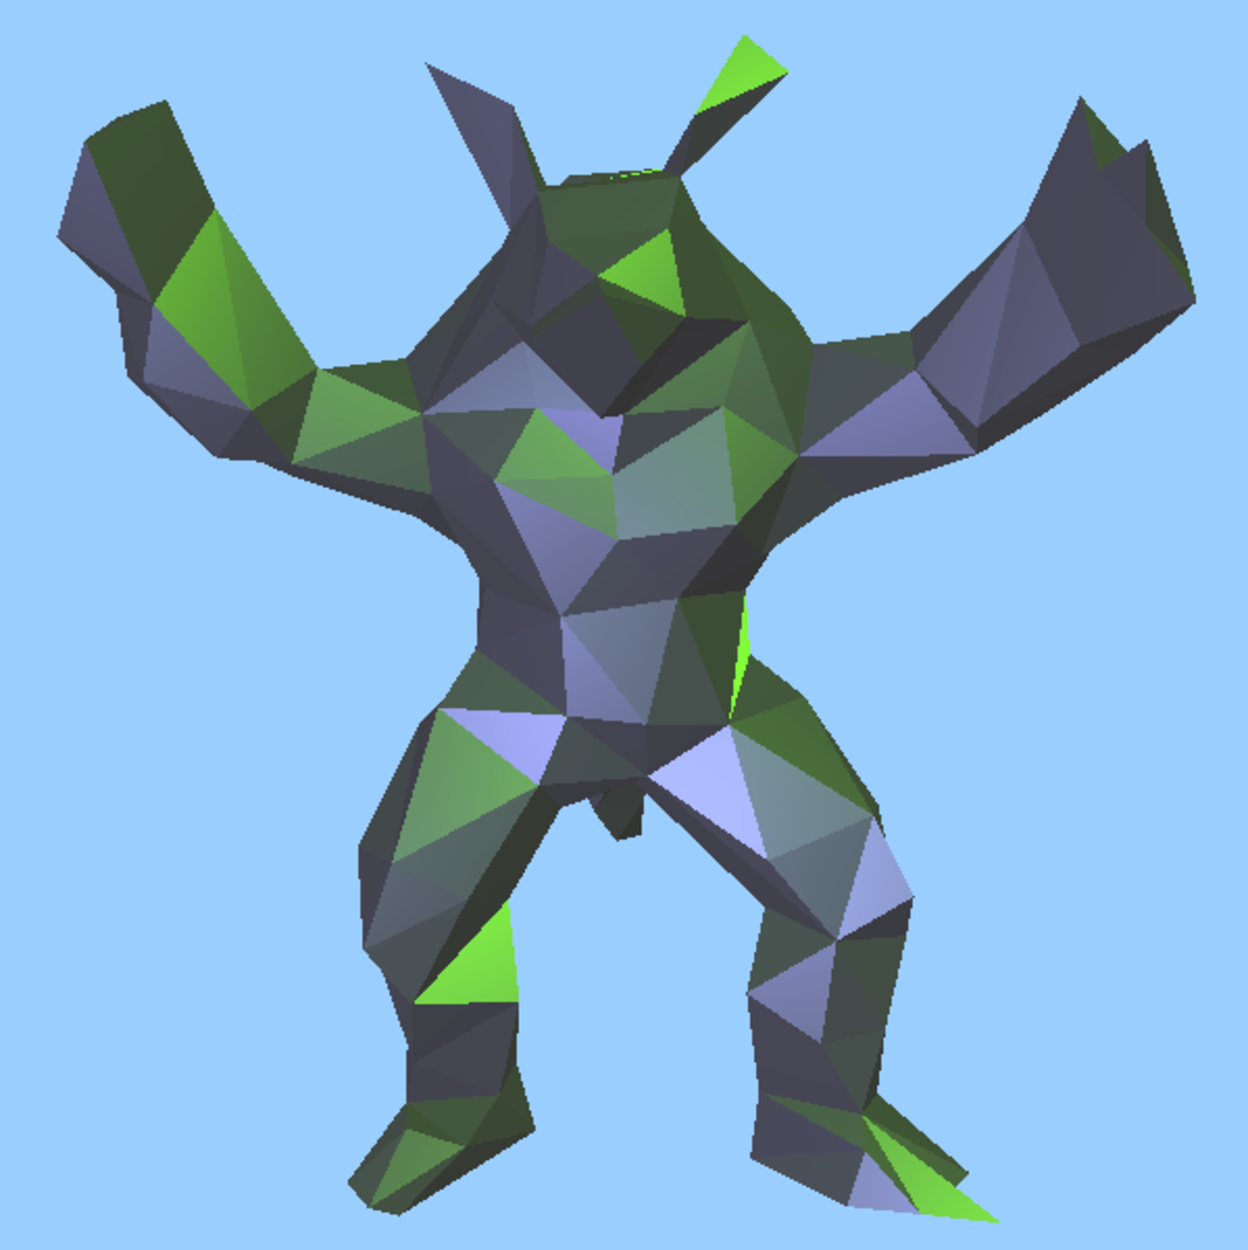
\includegraphics[width=.25\linewidth]{figs/armadillo376}
  \end{center}

\end{figure}


\end{document}
